\documentclass{standalone}
\usepackage{xcolor}
\usepackage{verbatim}
\usepackage[T1]{fontenc}
\usepackage{graphics}
\usepackage{hyperref}
\newcommand{\code}[1]{\texttt{#1}}
\newcommand{\R}{R}
\newcommand{\pkg}[1]{#1}
\newcommand{\CRANpkg}[1]{\pkg{#1}}%
\newcommand{\BIOpkg}[1]{\pkg{#1}}
\usepackage{amsmath,amssymb,array}
\usepackage{booktabs}
\usepackage{tikz}
\usetikzlibrary{arrows,positioning,shapes.geometric}
\usetikzlibrary{calc}
\usepackage[normalem]{ulem}
\usepackage{mathtools}
\usepackage{graphicx}
\usepackage{makecell}
\usepackage{bm}

\begin{document}
\nopagecolor
\centering
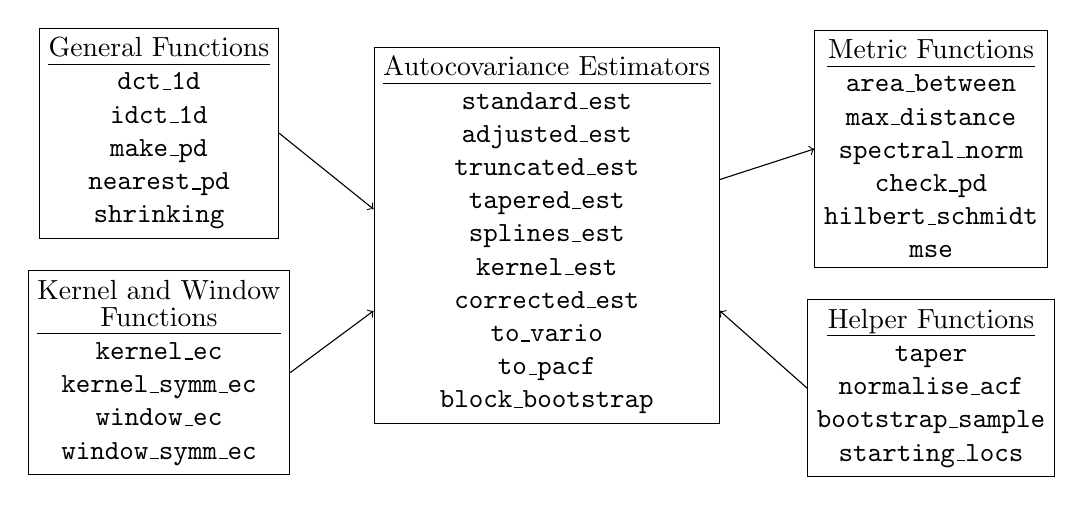
\begin{tikzpicture}
    \tikzstyle{block} = {draw, rectangle, align=center, minimum width=2cm, minimum height=1cm}
    \tikzstyle{line} = [draw, -latex']
    % Center
    \node [block,align=center]  (cov_ests) {\uline{Autocovariance Estimators}\\
        {\ttfamily standard\_est}\\
        {\ttfamily adjusted\_est}\\
        {\ttfamily truncated\_est}\\
        {\ttfamily tapered\_est}\\
        {\ttfamily splines\_est}\\
        {\ttfamily kernel\_est}\\
        {\ttfamily corrected\_est}\\
        {\ttfamily to\_vario}\\
        {\ttfamily to\_pacf}\\
        {\ttfamily block\_bootstrap}};
    % LEFT (slightly up)
    \node [block, align=center, left = 1.2cm of cov_ests, yshift=1.3cm] (general) {\uline{General Functions}\\
        {\ttfamily dct\_1d}\\
        {\ttfamily idct\_1d}\\
        {\ttfamily make\_pd}\\
        {\ttfamily nearest\_pd}\\
        {\ttfamily shrinking}};
    % LEFT BELOW (also shifted up)
      \node [block, align=center, below = 0.4cm of general] (kernels) {\uline{\shortstack{Kernel and Window\\Functions}}\\
        {\ttfamily kernel\_ec}\\
        {\ttfamily kernel\_symm\_ec}\\
        {\ttfamily window\_ec}\\
        {\ttfamily window\_symm\_ec}};
    % RIGHT
  \node [block, align=center, right = 1.2cm  of cov_ests, yshift=1.1cm] (metrics) {\uline{Metric Functions}\\
        {\ttfamily area\_between}\\
        {\ttfamily max\_distance}\\ 
        {\ttfamily spectral\_norm}\\
        {\ttfamily check\_pd}\\
        {\ttfamily hilbert\_schmidt}\\
        {\ttfamily mse}};
       % RIGHT BELOW
 \node [block, align=center,  below = 0.4cm of metrics] (helpers) {\uline{Helper Functions}\\
        {\ttfamily taper}\\
        {\ttfamily normalise\_acf}\\
        {\ttfamily bootstrap\_sample}\\
        {\ttfamily starting\_locs}};
    % Arrows (anchored to left side of center block)
   \draw [<-] ($(cov_ests.north west)!0.43!(cov_ests.south west)$) -- (general.east);
\draw [<-] ($(cov_ests.north west)!0.7!(cov_ests.south west)$) -- (kernels.east);
 \draw [->] ($(cov_ests.north east)!0.43!(cov_ests.south east)$)(cov_ests) -- (metrics.west);
    \draw [<-] ($(cov_ests.north east)!0.7!(cov_ests.south east)$) -- (helpers.west);
\end{tikzpicture}
\end{document}
